%%%%%%%%%%%%%%%%%%%%%%%%%%%%%%%%%%%%%%%%%
% File: funder_report.tex --- DRAFT funder report (Blue Marine Foundation).
% Compile from clean/tex/:
%   xelatex funder_report && bibtex funder_report && xelatex funder_report && xelatex funder_report
%
% BASIS (confirmed): SAM-led. Main results are the SAM management procedure
% (assessment error; the manuscript's main arm). Perfect information is the
% no-assessment-error bound only. The previous funder deliverable
% (tex/report.tex, tex/abstract.tex; frozen) was perfect-information only,
% reference OM bh3; that change is in the "Changes since the previous report"
% box. Do not revert to a perfect-information-led report.
%
% TODO (user): grant/contract reference, funder report template (if any),
% reporting period, Blue Marine contact name, branding (tex/exec_summary.tex
% used Imperial branding; this draft is unbranded), author list.
% TODO (user): mackerel 100-iteration results are pending a decision on
% the SAM convergence rule; not reported here (flagged in text only).
% TODO (user): the saved 02.4.3 results file has no convergence table
% (samMcConv); convergence of the 100-iteration refits is not reported.
%
% Numbers: clean/data/results/03.0_metrics_window.csv (SAM single
% realisation, PI, open loop, Historical; srr = bhw),
% 03.0_metrics_rebuild.csv, 02.4.3_closedLoop_sam_mc.RData (samMcMetrics;
% share above trigger computed from closedLoopSamMC terminal SSB),
% 04.1_multiSRR_review.csv, data/om/eqls.RData (bhwR0),
% 02.4.1_sam.RData (samRatio). Previous-report values: tex/report.tex
% (bh3, PI), reproduced by the bh3 PI rows of 04.1_multiSRR_review.csv.
%%%%%%%%%%%%%%%%%%%%%%%%%%%%%%%%%%%%%%%%%
%!TEX program = xelatex
\documentclass[11pt,a4paper]{article}

\usepackage{fontspec}
\usepackage[margin=2.4cm]{geometry}
\usepackage{amsmath,amssymb}
\usepackage{booktabs}
\usepackage{tabularx}
\usepackage{graphicx}
\usepackage[table,svgnames]{xcolor}
\usepackage{natbib}
\usepackage{tikz}
\usetikzlibrary{arrows.meta,positioning,calc}
\usepackage{pgfplots}
\pgfplotsset{compat=1.17}
\usepackage[most]{tcolorbox}
\usepackage{enumitem}
\usepackage{caption}
\usepackage{titlesec}
\usepackage{fancyhdr}
\usepackage{setspace}
\usepackage[colorlinks=true,linkcolor=NavyBlue,citecolor=NavyBlue,urlcolor=NavyBlue]{hyperref}

\definecolor{bmblue}{RGB}{0,62,116}
\definecolor{bmlight}{RGB}{232,240,248}
\definecolor{bmamber}{RGB}{255,244,224}
\definecolor{armhist}{RGB}{40,40,40}
\definecolor{armol}{RGB}{0,114,178}
\definecolor{armsam}{RGB}{213,94,0}
\definecolor{armpi}{RGB}{230,159,0}

\setstretch{1.1}
\setlength{\parindent}{0pt}
\setlength{\parskip}{0.55em}
\setlist{topsep=0.2em,itemsep=0.15em,leftmargin=1.3em}
\captionsetup{font=small,labelfont={bf,color=bmblue}}
\titleformat{\section}{\color{bmblue}\Large\bfseries}{\thesection}{0.6em}{}
\titleformat{\subsection}{\color{bmblue}\large\bfseries}{\thesubsection}{0.6em}{}

\pagestyle{fancy}
\fancyhf{}
\renewcommand{\headrulewidth}{0.3pt}
\fancyhead[L]{\small\color{bmblue}Backtest of ICES advice: Celtic and Irish Sea gadoids}
\fancyhead[R]{\small\color{bmblue}DRAFT for Blue Marine Foundation}
\fancyfoot[C]{\small\thepage}

\newtcolorbox{keybox}[1]{colback=bmlight,colframe=bmblue,fonttitle=\bfseries,
  title=#1,arc=1mm,boxrule=0.6pt,left=6pt,right=6pt,top=4pt,bottom=4pt,breakable}
\newtcolorbox{changebox}[1]{colback=bmamber,colframe=DarkOrange,fonttitle=\bfseries,
  coltitle=black,title=#1,arc=1mm,boxrule=0.6pt,left=6pt,right=6pt,top=4pt,bottom=4pt,breakable}

\newcommand{\Btrig}{B_{\mathrm{trigger}}}
\newcommand{\Blim}{B_{\mathrm{lim}}}
\newcommand{\Ftar}{F_{\mathrm{target}}}
\newcommand{\Bmsy}{B_{\mathrm{MSY}}}

\begin{document}

%==============================================================================
\thispagestyle{empty}
\begin{center}
{\color{bmblue}\LARGE\bfseries Would following the ICES advice rule have\\[0.2em]
rebuilt Celtic and Irish Sea cod and whiting?\par}
\vspace{0.6em}
{\large A historical backtest of the ICES Category~1 advice rule\par}
\vspace{1.0em}
{\large Report to the Blue Marine Foundation --- \textbf{draft for review}\par}
\vspace{0.8em}
Laurence T.~Kell, Sea++ \quad\textperiodcentered\quad \texttt{laurie@kell.es}\\[0.2em]
\small Grant reference: [to be supplied] \quad\textperiodcentered\quad 27 September 2026
\end{center}
\vspace{0.5em}

%==============================================================================
\section*{Executive summary}
\addcontentsline{toc}{section}{Executive summary}

Four gadoid stocks in the Celtic and Irish Seas are all below the ICES
biomass limit in the latest assessments: Celtic Sea cod, Irish Sea
whiting, Irish Sea cod and Celtic Sea whiting. The usual explanations are
that scientific advice was not followed, that the advice rule itself is not
good enough, or that the stocks became less productive. This project asked
which of these explanations the evidence supports. To answer it we
\emph{replayed history}: in a simulation that keeps each stock's actual
growth, natural mortality and recruitment history, we applied the ICES
advice rule every year from 2015, using a yearly stock assessment
fitted to simulated survey data (so the rule sees the stock with realistic
error), and compared the result with what actually happened.

\begin{keybox}{Key messages}
\begin{enumerate}[leftmargin=1.4em]
\item \textbf{Following the rule would have rebuilt the two overfished stocks.}
Fishing on Celtic Sea cod and Irish Sea whiting averaged about four to
five times the ICES target. Had the advice rule been followed from 2015,
both would have ended the period at about three times the ICES biomass
trigger (3.2 and 3.6) instead of far below it (0.02 and 0.68).
\item \textbf{For Irish Sea cod the rule would not have helped.} Fishing was
already well below the target, so the rule as written would have
\emph{allowed more} catch and left the stock slightly lower (0.41 instead
of 0.54 of the trigger). Its decline is not explained by overfishing
relative to the target.
\item \textbf{For Celtic Sea whiting the rule helps but does not rebuild.}
The rule roughly doubles the end-of-period stock (0.48 instead of 0.22 of
the trigger), but under the recruitment that actually occurred the stock
stays below the trigger.
\item \textbf{``Above the trigger'' is not the same as ``at MSY''.}
The ICES trigger and the stock size that gives maximum sustainable yield
(MSY) disagree, in both directions. For Celtic Sea cod and Irish Sea
whiting, MSY biomass is about four times the trigger, so clearing the
trigger is not full recovery. For Celtic Sea whiting the opposite holds.
\item \textbf{These conclusions are robust.} They hold without assessment
error, across 100 repeat runs with different survey noise, and across seven
alternative assumptions about how recruitment depends on stock size.
The size of the gains depends on those assumptions; the direction does not.
\end{enumerate}
\end{keybox}

\begin{changebox}{Changes since the previous report}
\begin{itemize}
\item \textbf{Main results now include assessment error.} The previous
report let the advice rule see the true stock size (``perfect
information''). The main results here use a yearly stock assessment (the
SAM state-space model) fitted to simulated survey data, as in the
peer-review manuscript. Perfect information is still shown, as the best
case with no assessment error.
\item \textbf{New reference operating model.} Recruitment in the simulated
stocks is now a Beverton--Holt curve whose ceiling equals the plateau of
the ICES hockey-stick at $\Blim$, following \citet{winker2026rebuilding}.
The previous curve (``bh3'') did not keep this scale. MSY biomass is
now defined at the ICES target fishing mortality, so the simulated stock
and the advice rule share one basis.
\item \textbf{Fair comparison with fixed fishing.} The constant-target
comparison now starts in 2015 from the same state as the advice rule,
rather than around 1990.
\item \textbf{Robustness added:} 100 repeat runs with assessment error, and
seven alternative recruitment curves. Celtic Sea haddock and Northeast
Atlantic mackerel are in the supplementary material.
\end{itemize}
Terminal stock size relative to the trigger under the advice rule, before
and after these changes:\\[0.3em]
\small
\begin{tabular}{@{}lccc@{}}
\toprule
 & Previous report & \multicolumn{2}{c}{This report (new operating model)} \\
\cmidrule(lr){3-4}
Stock & (perfect information, bh3) & Perfect information & With assessment (SAM) \\
\midrule
Celtic Sea cod     & 1.03 & 1.91 & \textbf{3.16} \\
Irish Sea whiting  & 2.03 & 3.26 & \textbf{3.58} \\
Irish Sea cod      & 0.42 & 0.41 & \textbf{0.41} \\
Celtic Sea whiting & 0.40 & 0.45 & \textbf{0.48} \\
\bottomrule
\end{tabular}\\[0.3em]
\normalsize
The first two outcome patterns reported previously are unchanged. The
third (ICES trigger versus MSY biomass) now points in both directions:
previously MSY biomass was below the trigger for all four stocks; now it is
about four times the trigger for Celtic Sea cod and Irish Sea whiting.
\end{changebox}

%==============================================================================
\section{What was asked and what has been delivered}
\label{sec:asked}

The proposal set four objectives: to \textbf{reconstruct} how each stock
was perceived each year, \textbf{reproduce} the advice rule,
\textbf{simulate} the stock under perfect implementation of the advice,
and \textbf{compare} that counterfactual with what actually happened. The
work was organised in four tasks (screening, assessment reconstruction,
counterfactual simulation, and analysis and reporting).
Table~\ref{tab:delivery} shows what was delivered against each.

\begin{table}[htbp]
\centering
\small
\caption{Delivery against the funded objectives and tasks.}
\label{tab:delivery}
\begin{tabularx}{\textwidth}{@{}p{3.6cm}p{1.9cm}X@{}}
\toprule
Objective / task & Status & What was done \\
\midrule
Task~1: Screening and benchmarks (5 days)
 & Delivered
 & Six candidate stocks screened (advice vs.\ catch, stock status);
   four gadoids chosen as main case studies; haddock and mackerel
   retained for the supplement. Delivered as a separate screening
   report. \\
Objective~1 / Task~2: Reconstruct yearly assessments (20 days)
 & Delivered by an alternative route
 & ICES archives hold past assessment \emph{outputs} but not the input data
   needed to re-run them year by year. Instead, a stock assessment (SAM)
   is re-fitted every simulated year to simulated survey and catch data.
   This reproduces the \emph{effect} of assessment error on advice, but not
   the specific errors made in each historical year. \\
Objective~2: Reproduce the advice rule
 & Delivered
 & ICES Category~1 MSY rule for the gadoids, including the $\pm20\%$ limit
   on year-to-year change in catch advice when the stock is above the
   trigger. The latest published ICES reference points are used
   throughout. For mackerel the Coastal States strategy was not coded;
   the ICES rule is applied as a counterfactual. \\
Objective~3 / Task~3: Simulate perfect implementation (15 days)
 & Delivered
 & Catch equals the advice every year. Run with assessment error (main
   result), with perfect information (best case), with 100 repeat runs, and
   with seven recruitment assumptions. \\
Objective~4 / Task~4: Compare and report (10 days)
 & Delivered (this report)
 & Stock status, fishing pressure, catch, catch stability and rebuilding
   time, for each stock and across stocks; peer-review manuscript,
   supplement and reproducible code (Section~\ref{sec:outputs}). \\
\bottomrule
\end{tabularx}
\end{table}

%==============================================================================
\section{Approach in plain terms}
\label{sec:approach}

\paragraph{What a backtest is.} A backtest asks ``what would have happened
if\dots?'' about the past. We build a computer model of each stock from its
latest ICES assessment, and keep everything that nature did the same: how
fast fish grew, how many died naturally, and how good or bad each year's
recruitment was relative to what the stock size would predict. The only
thing that changes is how the fishery was managed. Any difference in
outcome can then be put down to management rather than to luck with
recruitment or the environment.

\paragraph{The ICES advice rule.} ICES sets a target fishing pressure
($\Ftar$) and a biomass \emph{trigger} ($\Btrig$). If the spawning stock
is above the trigger, the advice is to fish at the target; below the
trigger, fishing is cut in proportion to how far the stock has fallen.
A lower biomass \emph{limit} ($\Blim$) marks where recruitment is thought
to be impaired. We report stock size as a ratio to the trigger: 1 means at
the trigger, below 1 means below it.

\paragraph{What is compared.} Each stock is run four ways from 2015 to its
latest assessment year (2023--2025), then 20 years ahead
(Figure~\ref{fig:design}):
\begin{itemize}
\item \textbf{Historical} --- what actually happened, from the latest ICES
assessment.
\item \textbf{Fixed fishing at the target (open loop)} --- fishing held at
the ICES target every year, ignoring stock size. This is a reference
point, not a management option.
\item \textbf{Advice rule with assessment (main result)} --- each year a
survey is simulated from the model stock, the SAM stock assessment is
fitted, the ICES rule sets next year's catch, and that catch is taken
exactly.
\item \textbf{Advice rule with perfect information (best case)} --- as
above, but the rule sees the true stock size, so there is no assessment
error.
\end{itemize}

\begin{figure}[htbp]
\centering
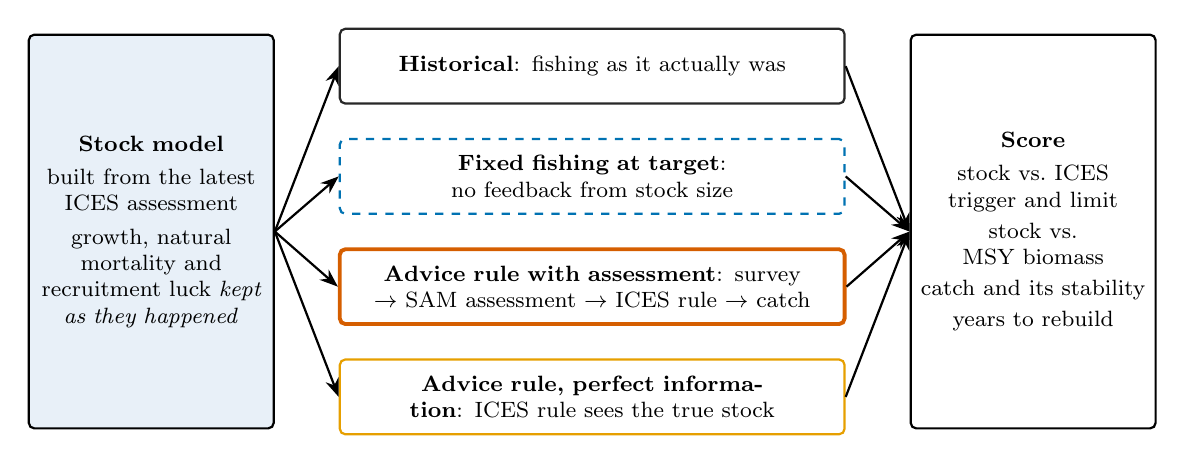
\begin{tikzpicture}[font=\footnotesize,>=Stealth,
  box/.style={draw,thick,rounded corners=2pt,align=center,inner sep=3pt},
  arm/.style={box,text width=6.2cm,minimum height=0.95cm}]
  \node[arm,draw=armhist] (h) at (0,2.1)
    {\textbf{Historical}: fishing as it actually was};
  \node[arm,draw=armol,dashed] (o) at (0,0.7)
    {\textbf{Fixed fishing at target}: no feedback from stock size};
  \node[arm,draw=armsam,line width=1.4pt] (s) at (0,-0.7)
    {\textbf{Advice rule with assessment}: survey $\rightarrow$ SAM
     assessment $\rightarrow$ ICES rule $\rightarrow$ catch};
  \node[arm,draw=armpi] (p) at (0,-2.1)
    {\textbf{Advice rule, perfect information}: ICES rule sees the true
     stock};
  \node[box,text width=2.9cm,minimum height=5.0cm,fill=bmlight] (om) at (-5.6,0) {%
    \textbf{Stock model}\\[0.3em]
    built from the latest ICES assessment\\[0.3em]
    growth, natural mortality and recruitment luck \emph{kept as they
    happened}};
  \node[box,text width=2.9cm,minimum height=5.0cm] (sc) at (5.6,0) {%
    \textbf{Score}\\[0.3em]
    stock vs.\ ICES trigger and limit\\[0.2em]
    stock vs.\ MSY biomass\\[0.2em]
    catch and its stability\\[0.2em]
    years to rebuild};
  \foreach \n in {h,o,s,p} {
    \draw[->,thick] (om.east) -- (\n.west);
    \draw[->,thick] (\n.east) -- (sc.west);
  }
\end{tikzpicture}
\caption{Design of the backtest. All four versions share the same stock
model and the same recruitment history; only the way fishing is set
differs.}
\label{fig:design}
\end{figure}

\paragraph{Two yardsticks.} Results are scored against the ICES trigger and
limit, and also against the stock size that would give maximum sustainable
yield (MSY biomass, $\Bmsy$). These are different quantities. The trigger
is a management threshold, chosen to be precautionary. MSY biomass is the
long-term stock size when fishing at the target. Managers and the public
often treat ``above the trigger'' as ``at MSY''
\citep{winker2026rebuilding}; the backtest tests whether that is true for
these stocks.

\paragraph{What stays fixed.} The ICES reference points are the latest
published values, not the ones in force in each year. The rule is applied
exactly as written (a small minimum fishing mortality remains below the
limit rather than a closure). Catch is taken exactly as advised, with no
overshoot. The single-species rule is applied to each stock separately,
without interactions between fleets and species.

%==============================================================================
\section{The four case studies}
\label{sec:stocks}

All four stocks are below the ICES limit $\Blim$ in the latest
assessments, but for different reasons. Fishing on Celtic Sea cod and Irish
Sea whiting was far above the target. Fishing on Irish Sea cod has been
below the target since about 2000, yet the stock still declined. Celtic
Sea whiting was fished above the target for most of the period and below
it in the latest year. Reported catches exceeded ICES advice in most
years since 2019--2020 for all four stocks (Figure~\ref{fig:advice}).

\begin{figure}[htbp]
\centering
\includegraphics[width=0.82\textwidth]{figs/advice_catch_casestudy.pdf}
\caption{ICES advised catch (blue, dashed) and reported catch (orange) for
the four case-study stocks, 2010 onward. Where catch is above advice,
advice was not fully implemented. Each panel has its own scale (tonnes).}
\label{fig:advice}
\end{figure}

%==============================================================================
\section{Results}
\label{sec:results}

\subsection{Three outcome patterns}

Figure~\ref{fig:terminal} summarises the main result: stock size at the
end of each stock's backtest period, relative to the ICES trigger, under
each version. Figure~\ref{fig:traj} shows the full trajectories.

\begin{figure}[htbp]
\centering
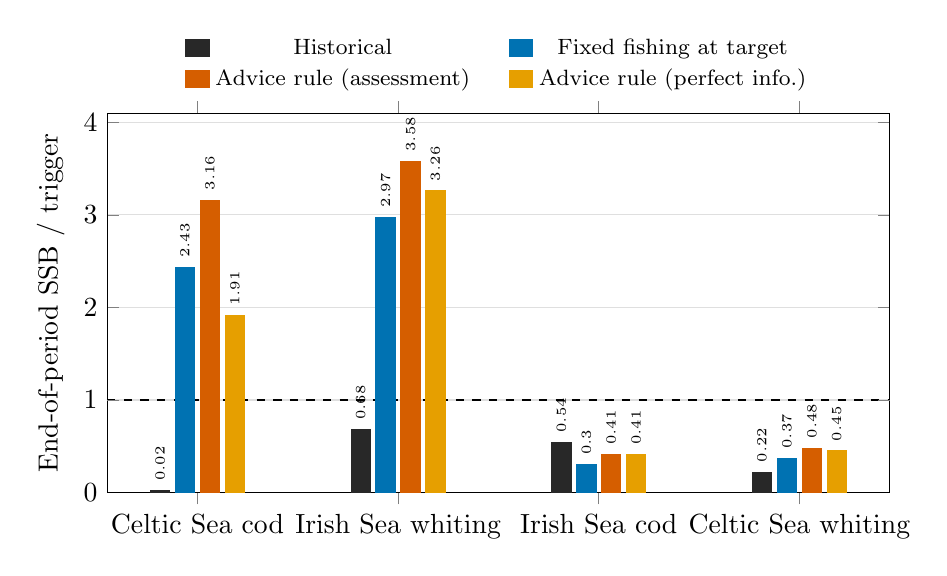
\begin{tikzpicture}
\begin{axis}[
  ybar, bar width=7pt, width=0.95\textwidth, height=6.4cm,
  ymin=0, ymax=4.1, ylabel={End-of-period SSB / trigger},
  symbolic x coords={CScod,ISwhg,IScod,CSwhg},
  xticklabels={Celtic Sea cod,Irish Sea whiting,Irish Sea cod,Celtic Sea whiting},
  xtick=data, enlarge x limits=0.15,
  legend style={at={(0.5,1.03)},anchor=south,legend columns=2,font=\footnotesize,draw=none,
    /tikz/every even column/.append style={column sep=1.2em}},
  legend image code/.code={\draw[#1] (0cm,-0.1cm) rectangle (0.3cm,0.12cm);},
  nodes near coords, every node near coord/.append style={font=\tiny,rotate=90,anchor=west},
  nodes near coords style={/pgf/number format/fixed,/pgf/number format/precision=2},
  ymajorgrids, grid style={gray!25},
  extra y ticks={1}, extra y tick labels={}, extra y tick style={grid=major,
    major grid style={black,dashed,thick}},
]
\addplot[fill=armhist,draw=armhist] coordinates {(CScod,0.02) (ISwhg,0.68) (IScod,0.54) (CSwhg,0.22)};
\addplot[fill=armol,draw=armol] coordinates {(CScod,2.43) (ISwhg,2.97) (IScod,0.30) (CSwhg,0.37)};
\addplot[fill=armsam,draw=armsam] coordinates {(CScod,3.16) (ISwhg,3.58) (IScod,0.41) (CSwhg,0.48)};
\addplot[fill=armpi,draw=armpi] coordinates {(CScod,1.91) (ISwhg,3.26) (IScod,0.41) (CSwhg,0.45)};
\legend{Historical, Fixed fishing at target, Advice rule (assessment), Advice rule (perfect info.)}
\end{axis}
\end{tikzpicture}
\caption{End-of-period spawning stock biomass (SSB) relative to the ICES
trigger (dashed line at 1) for 2015 to 2025 (Celtic Sea cod), 2023 (Irish
Sea stocks) and 2024 (Celtic Sea whiting). ``Advice rule (assessment)'' is
one simulated survey realisation.}
\label{fig:terminal}
\end{figure}

\begin{figure}[htbp]
\centering
\includegraphics[width=\textwidth]{figs/traj_facet_sam.pdf}
\caption{Historical (black) and advice-rule-with-assessment (orange)
trajectories of fishing mortality, SSB, recruitment and catch (rows) for
each stock (columns). Shading marks the period before 2015, the backtest
period, and the 20-year projection. Dashed lines are the ICES target
fishing mortality and the ICES trigger and limit; dotted grey lines are
MSY reference points.}
\label{fig:traj}
\end{figure}

\paragraph{Pattern 1: the rule would have rebuilt the two overfished stocks.}
Fishing on Celtic Sea cod and Irish Sea whiting averaged 3.9 and 4.7 times
the ICES target over the backtest period. Under the advice rule, fishing
fell sharply in the first years and rose back towards the target as the
stocks recovered. Both stocks would have ended about three times above the
trigger (3.16 and 3.58) rather than far below it (0.02 and 0.68). Years
with the stock below the limit fall from 9 of 11 to 2 (Celtic Sea cod) and
from 9 of 9 to 2 (Irish Sea whiting). The cost for Irish Sea whiting is
lower catch over the period (6.2 thousand tonnes instead of 11.0). For
Celtic Sea cod catch is higher (28.8 instead of 19.7 thousand tonnes)
because the stock recovers within the period. In both cases catch varies
more from year to year (on average 64\% and 58\% change per year, against
34\% and 25\% historically).

\paragraph{Pattern 2: opposite sign for Irish Sea cod.} Fishing on Irish Sea
cod averaged only 0.11 of the target. The rule, as written, would have
raised fishing towards the target, taking more catch (5.0 instead of 1.7
thousand tonnes) and leaving the stock slightly lower (0.41 instead of
0.54 of the trigger). Years below the limit are unchanged (2 of 9).
Low realised fishing may reflect advice that was stricter than the coded
rule, recovery measures, or catch limits set by other species in the
mixed fishery; the backtest cannot tell these apart.

\paragraph{Celtic Sea whiting: the rule helps but does not rebuild.}
Fishing averaged twice the target. The rule cuts it to 0.79 of the target
and roughly doubles the end-of-period stock (0.48 instead of 0.22 of the
trigger), but the stock is below the trigger in 9 of 10 years (as
historically), and below the limit in 7 of 10 (8 historically). Fixed fishing at the target does
no better (0.37). With the recruitment that actually occurred, no version
clears the trigger.

\paragraph{Pattern 3: the ICES trigger and MSY biomass disagree, in both directions.}
On the reference operating model, MSY biomass is 4.1 times the trigger for
Celtic Sea cod, 4.3 for Irish Sea whiting, 1.1 for Irish Sea cod and 0.77
for Celtic Sea whiting. So:
\begin{itemize}
\item For Celtic Sea cod and Irish Sea whiting, clearing the trigger is
\emph{not} full recovery. Under the advice rule they end at 0.77 and 0.83
of MSY biomass. In the 20-year projection Irish Sea whiting reaches MSY
biomass after 3 more years; Celtic Sea cod approaches it but does not
reach it within 20 years.
\item For Celtic Sea whiting the reverse holds. The stock reaches MSY
biomass within 7 years of the end of the backtest but \emph{never} reaches the
trigger, because below the trigger the rule keeps fishing below target
and the stock settles between the two.
\item For Irish Sea cod the two are close; the stock reaches the trigger
after 9 years but not MSY biomass within 20.
\end{itemize}

\paragraph{Does assessment error weaken the rule?} Not in these runs. The
results with the SAM assessment are close to, or better than, the
perfect-information best case. For the two overfished stocks, the
assessment-based rule cut fishing harder in the first years and so ended
with more fish (Celtic Sea cod 3.16 against 1.91). With perfect
information the true stock was above the trigger in 2015, so the
$\pm20\%$ limit on catch changes held catch close to its historical level
at first. The price of the deeper cuts was lower catch and greater
year-to-year variation in catch.

\subsection{Robustness to assessment error: 100 repeat runs}

The main results use one simulated survey. To check that they are not a
lucky draw, the assessment-based rule was run 100 times with different
survey noise, using a noisier survey (30\% error, against 10\% in the
single run). Figure~\ref{fig:iter} shows the spread.

\begin{figure}[htbp]
\centering
\includegraphics[width=0.95\textwidth]{figs/02.4.3_closedLoop_sam_mc-traj-ribbon-1.png}
\caption{Advice rule with assessment over 100 survey realisations (orange
line, labelled ``bhw'' after the reference operating model: median; band:
5--95\% range) against Historical (black), shown
relative to each stock's historical mean. Columns are stocks (including
Celtic Sea haddock, Section~\ref{sec:other}); rows are fishing mortality,
SSB, recruitment and catch. The dotted line marks 2015.}
\label{fig:iter}
\end{figure}

\begin{itemize}
\item \textbf{Irish Sea whiting:} median end-of-period stock 3.77 times the
trigger (5--95\% range 3.59--3.99); every run ends above the trigger.
\item \textbf{Celtic Sea cod:} median 2.87 (0.09--6.10). Starting from a
stock at 2\% of the trigger, outcomes are very sensitive to how well the
first assessments estimate that stock: 57 of 100 runs end above the
trigger. At least 95\% of runs still end above the historical outcome
(0.02).
\item \textbf{Irish Sea cod:} median 0.40 (0.34--0.43). At least 95\% of
runs end below the historical outcome (0.54), confirming Pattern~2.
\item \textbf{Celtic Sea whiting:} median 0.47 (0.33--0.59). No run
reaches the trigger, but at least 95\% improve on history (0.22).
\end{itemize}
Mackerel repeat runs are pending a decision on how to treat assessment fits
that do not converge, and are not reported here.

\subsection{Robustness to the recruitment assumption: seven curves}

How recruitment responds to stock size is uncertain, and it drives both
how fast a stock can rebuild and where MSY biomass sits. The backtest was
repeated with seven recruitment curves: the reference curve, three other
Beverton--Holt fits and three Ricker fits, with different constraints
(Figure~\ref{fig:srr}). Two pairs give practically identical results, so
there are effectively five distinct alternatives.

\begin{figure}[htbp]
\centering
\includegraphics[width=0.85\textwidth]{figs/04.1_multiSRR_review-heat-delta-1.png}
\caption{Change in end-of-period SSB/trigger from following the advice
rule (advice rule minus Historical) for each stock (rows) and recruitment
curve (columns; ``bhw'' is the reference). Top: perfect information;
bottom: with assessment (one survey realisation). Positive means the rule
would have left more fish.}
\label{fig:srr}
\end{figure}

No recruitment curve reverses any pattern. With the assessment-based rule,
the gain for Celtic Sea cod ranges from $+2.2$ to $+9.6$ trigger units and
for Irish Sea whiting from $+1.8$ to $+8.0$. Irish Sea cod is always
slightly worse under the rule ($-0.11$ to $-0.13$). Celtic Sea whiting always
gains a little ($+0.21$ to $+0.33$) but never reaches the trigger (at most
0.55). The recruitment curve changes \emph{how much} the rule would have
helped, not \emph{whether} it helps. It matters much more for the MSY
yardstick. Depending on the curve, MSY biomass ranges from 0.9 to 28 times the
trigger for Celtic Sea cod and from 0.14 to 1.3 for Irish Sea cod, so
Pattern~3 (which yardstick is harder to meet) depends on the recruitment
assumption. This is why the reference curve is tied to the ICES reference
points themselves.

\subsection{Beyond the case studies: haddock and mackerel}
\label{sec:other}

\paragraph{Celtic Sea haddock: a warning about lags.} Here assessment error
matters. With perfect information the rule ends the period at the trigger
(1.06); with the assessment it ends at 0.19, well below the historical
0.63. Recruitment collapsed in 2022. Because advice is based on an
assessment one year out of date, and the $\pm20\%$ limit on catch changes
applies while the stock is still assessed above the trigger, catches were
held up while the stock fell from 2022 (Figure~\ref{fig:had}). Across 100 repeat
runs the median is 0.11 (0.03--1.01), and only 6 of 100 runs end above the
trigger. The catch-stability clause can work against the stock when
recruitment fails suddenly.

\begin{figure}[htbp]
\centering
\includegraphics[width=0.62\textwidth]{figs/si/si_backtest_had.27.7b-k.pdf}
\caption{Celtic Sea haddock, 2015--2025: fishing mortality, SSB,
recruitment and catch under each version. The assessment-based rule (dark
orange) keeps catch high into the recruitment collapse, and fishing
mortality rises steeply at the end. The pink ``short-cut'' line is a
simplified assessment-error variant not discussed in this report.}
\label{fig:had}
\end{figure}

\paragraph{Northeast Atlantic mackerel: a counterfactual only.} Mackerel is
managed under the Coastal States long-term strategy, not the ICES
Category~1 rule, and its ICES assessment is not the simple SAM set-up used
here. Applying the ICES rule is therefore a ``what if'' rather than a test
of the management actually in place. In that ``what if'', the end-of-period
stock is almost the same in every version (0.77 historical; 0.77 with
assessment; 0.79 with perfect information).

%==============================================================================
\section{What this means}
\label{sec:meaning}

\paragraph{For management.}
\begin{itemize}
\item Where fishing ran far above the target (Celtic Sea cod, Irish Sea
whiting), \textbf{not following advice is enough to explain} why the stocks
are depleted. The advice rule, followed with realistic assessment error,
would have rebuilt them within the period.
\item Where fishing was already below the target (Irish Sea cod),
\textbf{``follow the advice'' is not the answer}. The single-stock rule would
have allowed more fishing. Explanations need to look at productivity,
mixed-fishery constraints, and whether the reference points fit the stock.
\item For Celtic Sea whiting, \textbf{the rule is not sufficient on its own}
to rebuild the stock under the recruitment that occurred.
\item \textbf{Clearing the trigger should not be reported as reaching MSY}.
For the two overfished stocks MSY biomass is about four times the trigger.
\item \textbf{Catch-stability rules have a cost.} They slowed the first cuts
for the overfished stocks under perfect information. For Celtic Sea
haddock, combined with a one-year lag in advice, they kept catches up during
a recruitment collapse.
\end{itemize}

\paragraph{For Blue Marine.} The backtest gives evidence-based answers
to the question ``would following scientific advice have prevented this?''
For Celtic Sea cod and Irish Sea whiting, yes, with a cost in catch and
catch stability for Irish Sea whiting. For Irish Sea cod and Celtic Sea
whiting, the answer is more nuanced, and messages about recovery would need
to address productivity and mixed fisheries as well as advice
compliance. The distinction between the ICES trigger and MSY biomass is
directly relevant to how stock recovery is described in public. The
method is reusable: it can be applied to any stock managed with a harvest
control rule for which an ICES-style assessment exists.

%==============================================================================
\section{Limitations}
\label{sec:limits}

\begin{itemize}
\item \textbf{No mixed-fishery modelling.} Each stock is managed on its own;
catch limits set by other species (``choke'' effects) are not modelled.
This matters most for Irish Sea cod.
\item \textbf{No historical assessment reconstruction.} The yearly
assessment is fitted to simulated data, not to the data actually available
each year, because those inputs are not archived. The backtest captures
the general effect of assessment error, not the specific historical
errors.
\item \textbf{SAM stands in for the Irish Sea cod assessment.} SAM is the
ICES assessment model for three of the four stocks, but not for Irish Sea
cod. A single test fit for Irish Sea cod did not converge, and it
estimated stock size 18\% low and fishing 21\% high. Irish Sea cod results
carry more assessment uncertainty than the others.
\item \textbf{Recruitment at very low stock size.} The recruitment curves do
not allow for recruitment collapsing faster than proportionally at very
low stock size (depensation). If that happens, the rebuilding of Celtic Sea
cod from 2\% of the trigger is optimistic.
\item \textbf{Fixed reference points and the rule as written.} The latest
ICES reference points are used for all years, and the rule does not close
the fishery below the limit, as issued advice sometimes did.
\item \textbf{Perfect implementation.} Catch always equals advice; the
backtest shows the potential of the rule, not what is achievable given
enforcement and discarding.
\end{itemize}

%==============================================================================
\section{Outputs delivered and next steps}
\label{sec:outputs}

\paragraph{Delivered.}
\begin{itemize}
\item \textbf{Peer-review manuscript} (in preparation): full methods and
results for the four case studies, with assessment error and perfect
information, and the recruitment-curve sensitivity.
\item \textbf{Supplementary material}: stock-by-stock figures for all six
stocks, including Celtic Sea haddock and Northeast Atlantic mackerel.
\item \textbf{Reproducible code}: data preparation, operating models,
backtests, metrics and figures, at
\url{https://github.com/laurieKell/backtest-ices}, with the backtest engine
at \url{https://github.com/laurieKell/FLBacktest}. The analysis can be
updated as new ICES assessments are published.
\item \textbf{This report} and the previous (perfect-information) report.
\end{itemize}

\paragraph{Next steps.}
\begin{enumerate}
\item Finalise and submit the manuscript, with the 100-iteration results
and the seven-curve sensitivity for the assessment-based rule.
\item Decide how to treat non-converging assessment fits, then report the
mackerel repeat runs.
\item Add a mixed-fishery (choke) scenario for Irish Sea cod and the
Celtic Sea gadoids.
\item Add a depensation scenario for the most depleted stocks
\citep{albertsen2025rebuilding}.
\item Where input data can be obtained from ICES working groups, replace the
simulated survey with true historical assessment reconstructions.
\end{enumerate}

\bibliographystyle{apalike}
\bibliography{refs}

\end{document}
